\section{HOLA}
\subsection{{La duración pulsos aumenta con la amplitud de modulación en el régimen oscilatorio del modelo determinista}
\subsectionmark{La duración del ciclo en el régimen oscilatorio}
\label{C5_sec:T_osc}


    
En el modelo conceptual que construimos de la dinámica de activación de ERK en ESCs, proponemos que las oscilaciones están controladas por la dosis de FGF4, que además controla la duración de los intervalos oscilatorios. En nuestras observaciones, tanto la duración de pulsos como el intervalo de interpulsado poseen escalas temporales similares, y sus valores modales parecen conservarse ante distintas dosis controladas de estímulo extracelular. Por esta razón creemos que una de las características distintivas de la dinámica que queremos describir es la duración de pulsos. En las distribuciones de duración de pulsos que medimos experimentalmente, observamos que tenían un valor modal definido, y un ancho determinado. A partir de obtener una expresión analítica para la duración de pulsos, buscamos especular sobre la posibilidad de que el modelo de fase con bifurcación de ciclo infinito y ruido blanco gaussiano que proponemos en el capítulo anterior pueda dar lugar a ese tipo de distribuciones. Esta expresión no sólo significa una contribución interesante para el área de sistemas estocásticos, sino que también nos permite estudiar su dependencia de los distintos parámetros de la descripción teórica, información relevante para entender las capacidades y limitaciones que el modelo propuesto tiene para describir la dinámica de actividad de ERK en ESCs que caracterizamos previamente en nuestros experimentos. 

Para construir esta expresión, comenzamos por deducir la expresión analítica de la duración de pulsos en el régimen oscilatorio del modelo determinista, expresión que fue calculada previamente. Luego, obtenemos una expresión para el régimen excitable, en donde consideramos una pequeña perturbación en el modelo determinista. Finalmente, calculamos la duración de pulsos en el modelo con ruido blanco gaussiano aditivo. 


Queremos calcular la duración de pulsos para el modelo de fase \ref{C5_eq:adler_determinista} en el régimen oscilatorio, donde $\alpha < \omega$. En un sistema dinámico oscilatorio, la duración de pulsos se corresponde con el período de oscilación $T_{\text{osc}}$ 
\begin{align}
    T_{\text{osc}}&= \int dt \\ 
    &= \int_{0}^{2 \pi} \frac{dt}{d\theta} d\theta \\
    &= \int_{0}^{2 \pi} \frac{1}{\omega + \alpha \sin{\theta}} d\theta.
    \label{C5_eq:T_osc_def}
\end{align}
Para resolver esta integral, proponemos el cambio de variables $z = e^{i \theta}$, donde $d\theta = \frac{1}{iz} dz$ y
\begin{align}
    \sin{\theta} = \frac{z - \overline{z}}{2}
                  = \frac{z^{2} - 1}{2} \cdot \frac{1}{z},
\end{align}
e integraremos en la circunferencia de radio unidad centrada en cero $C_{0,1}$. Luego, la expresión \ref{C5_eq:T_osc_def} queda como
\begin{align}
    T_{\text{osc}}&= \int_{0}^{2 \pi} \frac{1}{\omega + \alpha \sin{\theta}} d\theta \nonumber \\
    &= \frac{2}{\alpha} \oint_{C_{0,1}} \frac{1}{2 \frac{\omega}{\alpha} + \frac{z^{2} - 1}{z}} \; \frac{dz}{iz} \nonumber\\
    &= \frac{2}{i \alpha} \oint_{C_{0,1}} \frac{1}{2 \frac{z}{\delta} + z^{2}-1}dz,
    \label{C5_eq:T_osc_cambio_variables}
\end{align}
 donde definimos la variable adimensional $\delta = \frac{\alpha}{\omega}$. Para factorizar el denominador, es conveniente buscar sus ceros $z_\pm$
\begin{align}
    z_\pm^{2} + 2 \frac{z_\pm}{\delta} - 1=0 \nonumber\\
    z_\pm = -\frac{1}{\delta}  \pm \kappa
\end{align}
donde definimos $\kappa = \sqrt{1/\delta^{2} + 1}$. Con este resultado, es posible factorizar el denominador de la expresión \ref{C5_eq:T_osc_cambio_variables}, tal que 
\begin{equation}
    T_{\text{osc}}= \frac{2}{i \alpha} \oint_{C_{0,1}} \frac{1}{z-( -\frac{1}{\delta} + \kappa)} \; \frac{1}{z + (\frac{1}{\delta} + \kappa)} dz.
    \label{C5_eq:T_osc_factorizada}
\end{equation}
Para resolver la integral, utilizaremos el Teorema de los Residuos. Para implementar este teorema, es necesario primero localizar los polos, es decir, los valores de $z$ que anulan el denominador. Para el régimen oscilatorio de \ref{C5_eq:adler_determinista}, $\omega > \alpha $. Esta relación implica que $\frac{1}{\delta} >1$, y el polo correspondiente a $z_- = -\frac{1}{\delta}  - \kappa $ está fuera de la circunferencia $C_{0,1}$. En cambio, $\kappa - \frac{1}{\delta} < 1 $ y el polo correspondiente a $z_+$ se encuentra dentro de $C_{0,1}$. Esto demuestra que existe una sola singularidad aislada dentro de la región de integración, la circunferencia unitaria. El corolario del Teorema de Cauchy nos asegura que esta integral existe, y el Teorema de los Residuos nos conduce al siguiente resultado \cite{Strogatz1994}

\begin{align}
   T_{\text{osc}} &= \frac{2}{i\alpha} 2\pi i \lim_{z \to -\frac{1}{\delta} + \kappa} \frac{z-(-\frac{1}{\delta} + \kappa)}{[z-(-\frac{1}{\delta} + \kappa)][z + (\frac{1}{\delta} + \kappa)] } \label{ch4_eq:integracion_polos}\\
    &= \frac{4\pi}{\alpha} \lim_{z \to -\frac{1}{\delta} + \kappa} \frac{1}{z + (\frac{1}{\delta} + \kappa)} \nonumber \\
     &= \frac{4\pi}{\alpha}  \frac{1}{\frac{-1}{\delta} + \kappa + \frac{1}{\delta} + \kappa} \nonumber \\
     &=\frac{4\pi}{\alpha}  \frac{1}{2 \kappa} \nonumber\\
     &= \frac{2\pi}{\alpha \sqrt{\frac{1}{\delta^{2}} + 1}}. \nonumber
     \end{align}
Finalmente, 
\begin{align}
       T_{\text{osc}} &= \frac{2\pi}{\sqrt{\omega^{2}-\alpha^{2}}}.
      \label{C5_eq:T_osc}
\end{align}
Es decir, para el sistema dinámico descripto por la Ecuación de Adler la duración de pulsos en el régimen oscilatorio depende de sus dos parámetros $\alpha$ y $\omega$. Para independizarnos de la escala temporal, podemos escribir a $T_{\text{osc}}$ como
\begin{align}
    T_{\text{osc}} &= \frac{2\pi}{\omega} \times \frac{1}{\sqrt{1-\frac{\alpha^{2}}{\omega^{2}}}}.
\end{align}
El primer factor de esta expresión es el resultado para el oscilador uniforme, que se recupera cuando $\alpha = 0$. El segundo factor tiene origen en la no-homogeneidad del sistema. 


En la figura \ref{C5_fig:T_osc}A representamos la duración de pulsos en función del cociente entre la amplitud de modulación y la frecuencia del uniforme \dddelta para distintos valores de $\omega$. Observamos que la duración de pulsos aumenta conforme al aumento de \dddelta, y aumenta cuando disminuye la frecuencia del uniforme para valores fijos del cociente \dddelta. Este comportamiento evidencia que cuanto más aumenta la diferencia entre la frecuencia del uniforme y la amplitud de modulación (ya sea disminuyendo $\omega$ y manteniendo \dddelta fijo, o aumentando \dddelta con $\omega$ fijo), el sistema es cada vez menos uniforme y la duración de pulsos se vuelve más larga. A medida que disminuye la velocidad mínima y aumenta la velocidad máxima de la fase, el sistema pasa cada vez más tiempo en la región de velocidades mínimas, y menos en la de velocidades máximas. Este comportamiento conduce a un aumento en la duración de los pulsos \cite{Strogatz1994}. En los casos límites, cuando \dddelta se anula se recupera el resultado del oscilador uniforme, y en el límite donde $\alpha = \omega$ -cuando se produce la bifurcación de \textit{saddle-node} de ciclo infinito- la duración de pulsos es infinita. A continuación, queremos estudiar si esta tendencia se conserva en el régimen excitable. 


 \begin{figure}
    \centering
    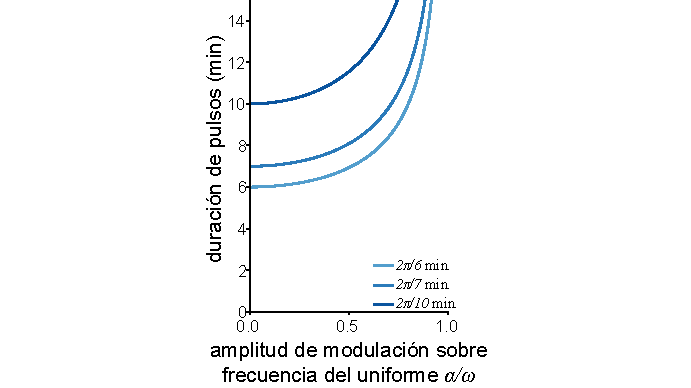
\includegraphics[width=1\columnwidth]{figures/chapter5/C5_T_osc.pdf} 
    \caption{\textbf{La duración de pulsos aumenta cerca de la bifurcación.} Duración de pulsos en función del cociente entre la amplitud de modulación y la frecuencia del uniforme \dddelta, para los valores de $\omega$ indicados.}
    \label{C5_fig:T_osc}
\end{figure}


\subsection{La duración del ciclo se reduce con la amplitud de modulación en el régimen excitable del modelo determinista}
\subsectionmark{La duración del ciclo en el régimen excitable}
\label{C5_sec:T_exc}

A continuación, nos proponemos calcular la duración de pulsos para el modelo de fase \ref{C5_eq:adler_determinista} en el régimen excitable, donde $\alpha > \omega$ y consideramos pequeñas perturbaciones que pueden dar lugar a actividad pulsátil. En este régimen hay un punto fijo inestable \xxi y un punto fijo estable \xxe, y el sistema tiende a permanecer en \xxe (figura \ref{C5_fig:adler_determinista_excitable}). Un ciclo de la fase \xx se consigue aplicando al sistema una perturbación mayor al umbral de excitabilidad, donde la fase sobrepasará el punto fijo inestable y hará una excursión antes de regresar al punto fijo estable. Esta excursión se traduce en un pulso de la señal $s(t)$ (ecuaciones \ref{C5_eq:seno_fase}, \ref{C5_eq:umbral}).



Entonces, formalmente definimos un \textbf{pulso en el régimen excitable} cuando el sistema sobrepasa \xxi y realiza una excursión hacia el punto fijo estable siguiente \xxe.\marginpar{duración de pulsos en el régimen excitable} La \textbf{duración de un pulso en el régimen excitable} $T_{\text{exc}}$ es, entonces, el tiempo que tarda el sistema en llegar a \xxe, habiendo partido de \xxi. Analíticamente, proponemos una definición análoga a la expresión \ref{C5_eq:T_osc_def}, 
\begin{align}
    T_{\text{exc}} = \int_{\xxi}^{\xxe}  \frac{1}{\omega + \alpha \sin{\xx}} d\xx. \label{C5_eq:T_exc_def}
\end{align}
En este caso, en lugar de integrar a lo largo de todo el círculo, fijamos los límites de integración en el punto fijo inestable \xxi y el punto fijo estable siguiente \xxe. Por simplicidad, elegimos $n_1,n_2 = 0$ en la definición \ref{C5_eq:PF_def}, y los límites de integración son
\begin{equation}
    \xxi = -\arcsin{\frac{\omega}{\alpha}} \quad \xxe = \pi + \arcsin{\frac{\omega}{\alpha}} \quad \text{para } \xxi,\xxe \in [-\frac{\pi}{2},\frac{3\pi}{2}).
\end{equation}
La región de integración está representada en la circunferencia trigonométrica de la figura \ref{C5_fig:T_exc_def}A. 


 \begin{figure}
    \centering
    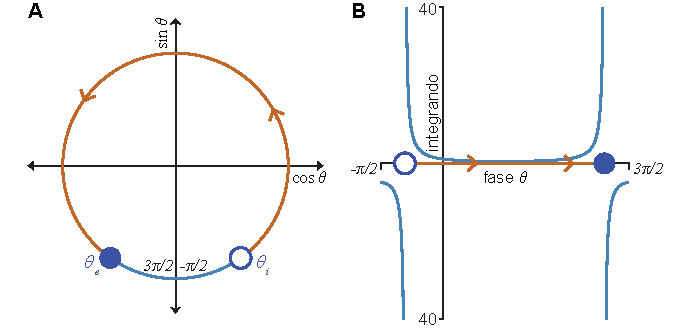
\includegraphics[width=1\columnwidth]{figures/chapter5/C5_T_exc_def.pdf} 
    \caption{\textbf{Definición de duración de pulsos para el régimen excitable.} (A) Trayectoria de la variable de integración en la circunferencia trigonométrica (azul). (B) Integrando de \ref{C5_eq:T_exc_def} en función de su variable de integración. (A,B) Se encuentran indicados los puntos fijos estable \xxe (círculo azul relleno) e inestable \xxi (círculo azul vacío). El intervalo de integración de la definición \ref{C5_eq:T_exc_def} está representando en naranja, y  las flechas naranjas indican la dirección de integración. Los límites del dominio del intervalo de integración están indicados. Parámetros: $\omega=2\pi/7\;min^{-1}$, $\alpha = 1.1 \times 2\pi/7\;min^{-1}$.}
    \label{C5_fig:T_exc_def}
\end{figure}


Por su definición formalizada en \ref{C5_eq:PF_def}, el denominador del integrando de \ref{C5_eq:T_exc_def} se anula en los puntos fijos. Esta propiedad conduce a que el integrando diverja en los límites de integración, y en consecuencia que la integral \ref{C5_eq:T_exc_def} diverja (figura \ref{C5_fig:T_exc_def}B). Este resultado es consecuencia de que el sistema tarda infinito tiempo en salir del punto fijo inestable. Proponemos salvar esta divergencia realizando la integral \ref{C5_eq:T_exc_def} en un entorno de los puntos fijos, tal que
\begin{align}
    T_{\text{exc}} = \int_{\xxi+\epsilon_\theta}^{\xxe-\epsilon_\theta}  \frac{1}{\omega + \alpha \sin{\xx}} d\xx \qquad \text{con } 0<\epsilon_\theta \ll 1.
    \label{C5_eq:T_exc_def_eps}
\end{align}
%Esta propuesta está representada en la figura PONER FIGURA. 
%VER SI LA CONVERGENCIA AL PUNTO FIJO ESTABLE ES ASINTOTICA O NO


Es útil reescribir la integral \ref{C5_eq:T_exc_def_eps} para obtener una expresión más sencilla de integrar. Primero efectuamos una traslación de la variable de integración \xx
\begin{align}
    \xx &= \gamma + \frac{\pi}{2} \qquad 
    d\xx = d\gamma. 
\end{align}
Con esta operación, trasladamos a los puntos fijos desde los cuadrantes $[-\frac{\pi}{2},\frac{3}{2} \pi)$ hacia $[-\pi, \pi)$. Los puntos fijos quedan simétricos respecto del cero (figura \ref{C5_fig:T_exc_T1}A), con valores
\begin{align}
    \gamma_i &= -\arcsin{\frac{\omega}{\alpha}} - \frac{\pi}{2} \qquad
    \gamma_e = \arcsin{\frac{\omega}{\alpha}} + \frac{\pi}{2}.
\end{align}
La integral \ref{C5_eq:T_exc_def_eps} queda escrita como (figura \ref{C5_fig:T_exc_T1}B)
\begin{align}
    T_{\text{exc}} = \int_{\gamma_i+\epsilon_\gamma}^{\gamma_e-\epsilon_\gamma}  \frac{1}{\omega + \alpha \cos{\gamma}} d\gamma \qquad \text{con } 0 < \epsilon_\gamma \ll 1.
    \label{C5_eq:T_exc_def_T1}
\end{align}

 \begin{figure}
    \centering
    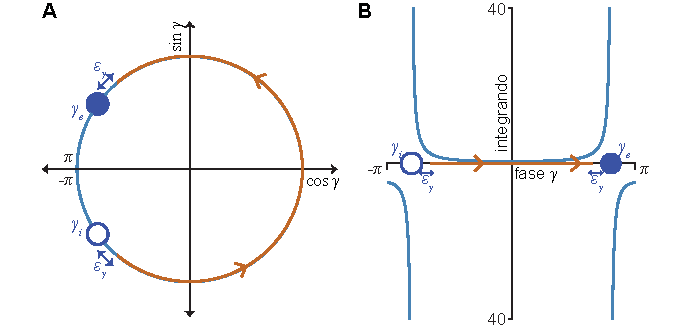
\includegraphics[width=1\columnwidth]{figures/chapter5/C5_T_exc_T1.pdf} 
    \caption{\textbf{Paso intermedio en el cómputo de la duración de pulsos para el régimen excitable.} (A) Trayectoria de la variable de integración en la circunferencia trigonométrica (azul). (B) Integrando de \ref{C5_eq:T_exc_def_T1} en función de su variable de integración. (A,B). Se encuentran indicados los puntos fijos estable \xxe (círculo azul relleno) e inestable \xxi (círculo azul vacío). El intervalo de integración está representando en naranja, y  las flechas naranjas indican la dirección de integración. A modo cualitativo, se indica $\epsilon_\gamma$. Se incluyen también los límites del dominio del intervalo de integración. Parámetros: $\omega=2\pi/7\;min^{-1}$, $\alpha = 1.1 \times 2\pi/7\;min^{-1}$.}
    \label{C5_fig:T_exc_T1}
\end{figure}

A continuación, realizamos la siguiente transformación de la variable de integración $\gamma$
\begin{align}
    \beta &= \frac{\gamma}{2} \qquad
    d\beta = \frac{d\gamma}{2}.
    \label{C5_eq:T_exc_T2}
\end{align}
Los valores de $\gamma$ se encuentran en el intervalo $[\gamma_i,\gamma_e] \in [-\pi, \pi)$. La transformación \ref{C5_eq:T_exc_T2} posiciona a los puntos fijos dentro del intervalo $[\frac{-\pi}{2},\frac{\pi}{2})$ (figura \ref{C5_fig:T_exc_T2}A), tal que
\begin{align}
    \gamma_i &= - \frac{1}{2} \arcsin{\frac{\omega}{\alpha}} - \frac{\pi}{4} \qquad
    \gamma_e  = \frac{1}{2} \arcsin{\frac{\omega}{\alpha}} + \frac{\pi}{4}.
\end{align}
La integral \ref{C5_eq:T_exc_def_T1} queda expresada como (figura \ref{C5_fig:T_exc_T2}B)
\begin{align}
    T_{\text{exc}} = \int_{\beta_i+\epsilon_\beta}^{\beta_e-\epsilon_\beta}  \frac{2}{\omega + \alpha \cos{2 \beta}} d\beta \qquad \text{con } 0< \epsilon_\beta \ll 1.
    \label{C5_eq:T_exc_def_T2}
\end{align}

 \begin{figure}
    \centering
    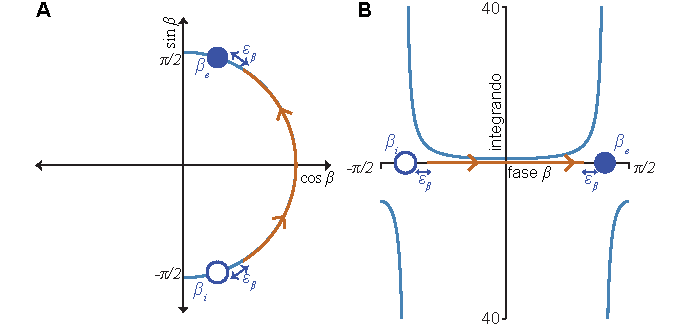
\includegraphics[width=1\columnwidth]{figures/chapter5/C5_T_exc_T2.pdf} 
    \caption{\textbf{Paso intermedio en el cómputo de la duración de pulsos para el régimen excitable.} (A) Trayectoria de la variable de integración en la circunferencia trigonométrica (azul). (B) Integrando de \ref{C5_eq:T_exc_def_T2} en función de su variable de integración. (A,B) Se encuentran indicados los puntos fijos estable \xxe (círculo azul relleno) e inestable \xxi (círculo azul vacío). El intervalo de integración está representando en naranja, y  las flechas naranjas indican la dirección de integración. A modo cualitativo, se indica $\epsilon_\beta$. Se incluyen también los límites del dominio del intervalo de integración. Parámetros: $\omega=2\pi/7\;min^{-1}$, $\alpha = 1.1 \times 2\pi/7\;min^{-1}$.}
    \label{C5_fig:T_exc_T2}
\end{figure}

Para terminar, transformamos la variable $\beta$ como
\begin{align}
    \lambda &= \tan{\beta} \qquad
    d\lambda = (1+\lambda^2) d\beta. 
    \label{C5_eq:T_exc_T3}
\end{align}
En el intervalo $[\frac{-\pi}{2},\frac{\pi}{2})$ donde está contenida la región de integración definida para $\beta$, la función tangente es biyectiva, lo que permite realizar el cambio de variables \ref{C5_eq:T_exc_T3}. Además es creciente, y el subespacio $[\frac{-\pi}{2},0)$ mapea a números negativos de $\lambda$, y $(0,\frac{\pi}{2}]$ a positivos. 


 \begin{figure}
    \centering
    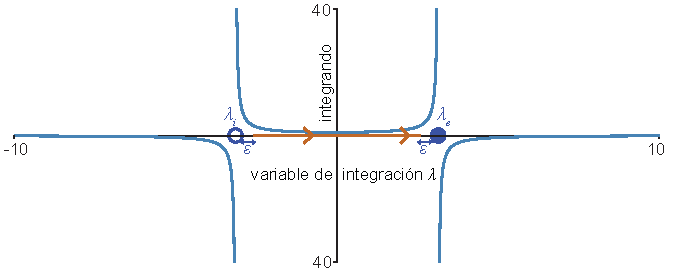
\includegraphics[width=1\columnwidth]{figures/chapter5/C5_T_exc_T3.pdf} 
    \caption{\textbf{Paso intermedio en el cómputo de la duración de pulsos para el régimen excitable.} Integrando de \ref{C5_eq:T_exc_def_T3} en función de su variable de integración. Se indican los puntos fijos estable \xxe (círculo azul relleno) e inestable \xxi (círculo azul vacío). El intervalo de integración está representando en naranja, y  las flechas naranjas indican la dirección de integración. A modo cualitativo, se indica $\epsilon$. Parámetros: $\omega=2\pi/7\;min^{-1}$, $\alpha = 1.1 \times 2\pi/7\;min^{-1}$.}
    \label{C5_fig:T_exc_T3}
\end{figure}


Ahora es necesario reescribir la integral \ref{C5_eq:T_exc_def_T2} en función de la nueva variable $\lambda$. Para reescribir el denominador, resultan útiles las relaciones trigonométricas
\begin{align}
    \cos{\beta} = \frac{1}{\sqrt{1+\lambda^2}} \quad \text{y} \quad \sin{\beta} = \frac{\lambda}{\sqrt{1+\lambda^2}}.
\end{align}
Luego,
\begin{align}
    \cos{2 \beta} &= \cos^2(\beta)-\sin^2(\beta)\\
    &=\frac{1}{1+\lambda^2} -  \frac{\lambda^2}{1+\lambda^2} \nonumber\\
    &= \frac{1-\lambda^2}{1+\lambda^2}.
\end{align}
Si incorporamos estas expresiones, la duración de pulsos queda expresada como
\begin{align}
    T_{\text{exc}} &= \int_{\lambda_i+\epsilon}^{\lambda_e -\epsilon} \frac{1}{\omega + \alpha \frac{1-\lambda^2}{1+\lambda^2}} \; \frac{2}{1+\lambda^2} d\lambda \\ 
    &= \frac{2}{\omega}\int_{\lambda_i+\epsilon}^{\lambda_e -\epsilon} d\lambda \frac{1}{1+\lambda^2+\ddelta \left(1-\lambda^2 \right)} \nonumber\\
    &= \frac{2}{\omega}\int_{\lambda_i+\epsilon}^{\lambda_e -\epsilon} d\lambda \frac{1}{\left(1+\ddelta \right) + \left( 1-\ddelta\right) \lambda^2} \qquad \text{con } 0<\epsilon \ll 1. \label{C5_eq:T_exc_def_T3}
\end{align}

La integral \ref{C5_eq:T_exc_def_T3} está representada en la figura \ref{C5_fig:T_exc_T3}. Para hacer frente a esta integral, nos falta encontrar expresiones para $\lambda_i$ y $\lambda_e$. Para esto, es conveniente recordar que, por definición, los puntos fijos \xxi y \xxe son quienes anulan el denominador en la expresión \ref{C5_eq:T_exc_def} de la duración de pulsos en el régimen excitable. Entonces, $\lambda_i$ y $\lambda_e$ son quienes anulan el denominador en \ref{C5_eq:T_exc_def_T3}, y buscamos $\lambda_i,\lambda_e$ tal que 
\begin{align}
    \left(1+\ddelta \right) + \left(1-\ddelta \right) \lambda_{e,i}^2 = 0\\
    \lambda_{e,i} = \pm \sqrt{\frac{1+\ddelta}{\ddelta-1}}. \label{C5_eq:PF_lambda}
\end{align}
En esta expresión, el punto fijo inestable es el menor y el estable el mayor en la expresión \ref{C5_eq:PF_lambda} (figura \ref{C5_fig:T_exc_T3}). Con este resultado, podemos realizar la integral \ref{C5_eq:T_exc_def_T3}, y
\begin{align}
    T_{\text{exc}} &= \frac{2}{\omega}\int_{\lambda_i + \epsilon}^{\lambda_e - \epsilon} d\lambda \frac{1}{\left(1+\ddelta\right) + \left(1-\ddelta\right) \lambda^2} \\
    &= \frac{2}{i\omega \sqrt{\ddelta^2 - 1}} \arctan{\left(i\sqrt{\frac{\ddelta - 1}{\ddelta + 1} } \lambda\right)} \Bigg]_{\lambda_i + \epsilon}^{\lambda_e - \epsilon} \nonumber\\
    &= \frac{2}{i \omega \sqrt{\ddelta^2 - 1}}  \left[ \arctan{\left( +i - i \epsilon \sqrt{\frac{\ddelta - 1}{\ddelta + 1}}\right)}  - \arctan{\left( -i +i \epsilon \sqrt{\frac{\ddelta - 1}{\ddelta + 1}}\right)} \right] \nonumber\\
    &= \frac{2}{\omega \sqrt{\ddelta^2 - 1}}  \frac{2}{i} \arctan{\left( i - i \epsilon \sqrt{\frac{\ddelta - 1}{\ddelta + 1}}\right)}.
\end{align}
Primero resolvimos la integral por tabla, luego reemplazamos los extremos de integración, y finalmente usamos que la tangente es impar para reescribir el resultado. Con esta expresión, podemos utilizar la expresión logarítmica de la forma compleja del arcotangente para embellecer la expresión que calculamos, y 
\begin{align}
    T_{\text{exc}} &= \frac{2}{\omega \sqrt{\ddelta^2 - 1}}  \frac{2}{i} \arctan{\left( i - i \epsilon \sqrt{\frac{\ddelta - 1}{\ddelta + 1}}\right)}\\ 
    &= \frac{-2}{ \omega \sqrt{\ddelta^2 - 1}}  \log{\left( \frac{\epsilon \sqrt{\frac{\dddelta - 1}{\dddelta + 1}}}{2-\epsilon \sqrt{\frac{\dddelta - 1}{\dddelta + 1}}}\right)}
\end{align}
Finalmente, la duración de pulsos en el régimen excitable es
\begin{align}
T_{\text{exc}} &=\frac{2\pi}{\sqrt{\alpha^2 - \omega^2}} \; \times \; -\frac{1}{\pi}  \log{\left( \frac{\epsilon \sqrt{\frac{\dddelta - 1}{\dddelta + 1}}}{2-\epsilon \sqrt{\frac{\dddelta - 1}{\dddelta + 1}}}\right)} \qquad \text{con } 0<\epsilon \ll 1.
    \label{C5_eq:T_exc}
\end{align}
Para verificar este resultado, medimos la duración de pulsos en el sistema dinámico descripto por la ecuación \ref{C5_eq:adler_determinista} en el régimen excitable. En estas mediciones determinamos cuánto tiempo tardaba el sistema en llegar a $\xxe-\epsilon$ dada su condición inicial $\xxi+\epsilon$ en series temporales $\theta(t)$ simuladas con la dinámica de la ecuación $\ref{C5_eq:adler_determinista}$. En la figura \ref{C5_fig:T_exc_res} observamos que el resultado analítico \ref{C5_eq:T_exc} es consistente con las simulaciones. 


Observamos que la duración de los pulsos en el régimen excitable se reduce conforme aumenta el cociente \ddelta (figura \ref{C5_fig:T_exc_res}). Un aumento en \ddelta conduce a mayores velocidades positivas que gobiernan las trayectorias del sistema dinámico desde \xxi hacia \xxe (ver eje $y$ en figura \ref{C5_fig:adler_determinista_excitable}A). Entonces, la reducción de la duración de pulsos es simplemente consecuencia de que el sistema dinámico se mueve más rápido desde \xxi hacia \xxe.  

Advertimos que la dependencia de $\epsilon$ se limita sólo a la función logarítmica, donde está contenida la divergencia, y que el factor que multiplica el logaritmo es una expresión análoga a la duración de pulsos en el caso oscilatorio \ref{C5_eq:T_osc}. Con la intención de resumir el resultado obtenido a partir esta observación, definimos 
\begin{equation}
    x = \epsilon \sqrt{\frac{\ddelta - 1}{\ddelta + 1}},
\end{equation}
y podemos reescribir el resultado \ref{C5_eq:T_exc} para valores pequeños de $\epsilon$ como
\begin{align}
    T_{\text{exc}} \simeq \frac{2\pi}{\sqrt{\alpha^2 - \omega^2}} \; \times \; -\frac{1}{\pi}  \log{\frac{x}{2}} \qquad \text{con } 0<x \ll 1.
    \label{C5_eq:T_exc_aprox}
\end{align}
Con esta expresión, es fácil ver que $T_{\text{exc}} \rightarrow +\infty$ cuando $\epsilon \rightarrow 0$ (y $x \rightarrow 0$). También observamos en la figura \ref{C5_fig:T_exc_res} que a mayores valores de $\epsilon$, disminuye sistemáticamente la duración de pulsos, como esperábamos.

 \begin{figure}
    \centering
    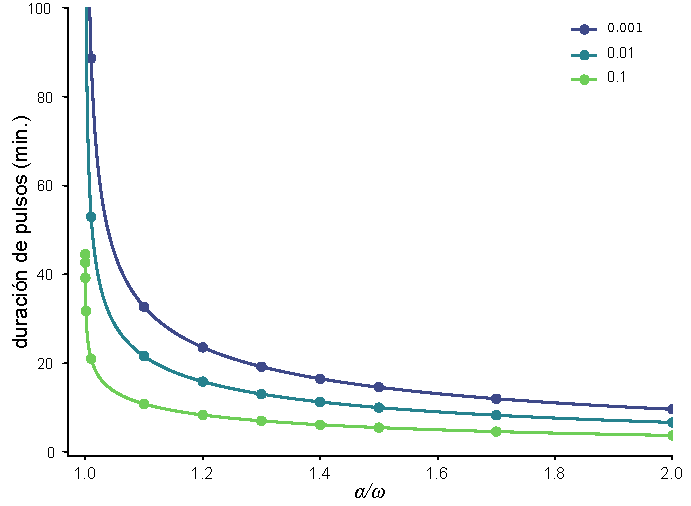
\includegraphics[width=1\columnwidth]{figures/chapter5/C5_T_exc.pdf} 
    \caption{\textbf{Duración de pulsos para oscilaciones no uniformes.} En escala de grises se grafica la duración de pulsos \ref{C5_eq:T_exc} en función del cociente entre la amplitud de modulación y la frecuencia del uniforme \ddelta para los valores de $\epsilon$ indicados. Los puntos de colores reportan las mediciones numéricas análogas (frecuencia de muestreo $0.00001\; min$). Parámetro: $\omega=2\pi/7\;min^{-1}$.}
    \label{C5_fig:T_exc_res}
\end{figure}



\section{La duración de pulsos depende de la intensidad del ruido}
\sectionmark{La duración de pulsos depende de ...}
\label{C6_sec:duracion}


Queremos obtener una expresión analítica de la duración de pulsos del sistema dinámico \ref{C6_eq:adler_white_noise}. Para el régimen excitable, en \ref{C5_sec:T_exc} definimos un pulso cuando el sistema sobrepasa el punto fijo inestable \xxi y realiza una excursión hacia el punto fijo estable siguiente \xxe, siendo su duración $T_{exc}$ el tiempo que tarda el sistema en llegar \emph{al entorno de} \xxe, habiendo partido \emph{del entorno de} \xxi. La versión estocástica \ref{C6_eq:adler_white_noise} tiene la ventaja de que no es necesario posicionarse en el entorno de los puntos fijos, pues es el ruido quien eventualmente perturbará al sistema y generará una excursión o pulso. Sin embargo, el carácter estocástico del sistema añade cierta complejidad al cálculo de este observable.

Para una sola trayectoria del sistema en el régimen excitable, podemos pensar a la duración de un pulso como el tiempo que tarda el sistema en alcanzar el punto fijo estable \xxe, dado que el comenzó en el punto fijo inestable \xxi y durante ese tiempo no volvió al punto fijo inestable \xxi. Como distintas posibles trayectorias del sistema pueden tener pulsos con distinta duración, la duración de pulsos es una variable aleatoria y su distribución de probabilidad asociada determina la posibilidad de que se den los diferentes valores. Para nuestros objetivos, es suficiente estudiar cómo depende la duración de pulsos media de la intensidad del ruido. Para obtener una expresión analítica de la duración de pulsos media, es útil trabajar con el tiempo de primer pasaje condicional medio. 


\marginpar{tiempo de\\primer pasaje\\condicional medio}
En el contexto de este problema, el tiempo de primer pasaje medio para un sistema estocástico es el tiempo medio que tarda el sistema en alcanzar un determinado umbral por primera vez, dada su condición inicial \cite{Redner2001}. De esta definición, el tiempo de primer pasaje condicional medio es el tiempo medio que tarda el sistema en alcanzar un determinado umbral de llegada por primera vez dada su condición inicial, y dado que no cruzó un umbral prohibido en el trayecto.  

\marginpar{duración de\\pulsos media}
En el régimen excitable, definimos \textbf{el tiempo de primer pasaje condicional medio} \tplus(\xx) como el tiempo que le toma al sistema alcanzar el punto fijo estable \xxe por primera vez, dado que salió de \xx y nunca pasó por el punto fijo inestable \xxi. Con esta idea, definimos la \textbf{duración de pulsos media} $T_\xi$ en el excitable como el tiempo medio que tarda el sistema en llegar a al punto fijo estable \xxe, habiendo salido pero nunca vuelto a pasar por el punto fijo inestable \xxi, es decir,
\begin{align}
    T_\xi = \lim_{\xx \rightarrow \xxi}\tplus(\xx).
    \label{C6_eq:Txi_def}
\end{align}.

Para el caso oscilatorio, es intuitivo pensar que la duración de pulsos media es el tiempo medio que tarda el sistema en alcanzar $\xx_0+2\pi$, habiendo salido y no vuelto a $\xx_0$. Este problema también es un problema de tiempo de primer pasaje condicional, y es trivial extender la definición \ref{C6_eq:Txi_def} a este régimen reemplazando $\xxi \rightarrow \xx_0$ y $\xxe \rightarrow \xx_0+2\pi$. Por simplicidad, trabajaremos con la notación \ref{C6_eq:Txi_def} más amigable para el régimen excitable, y luego haremos los reemplazos correspondientes para estudiar la duración de pulsos media en el régimen oscilatorio. 

Para obtener una expresión analítica de la duración de pulsos media, comenzaremos por obtener una expresión para el tiempo de primer pasaje condicional medio. Primero buscaremos obtener una ecuación diferencial para esta variable, y luego indagaremos sobre su solución. Finalmente, tomaremos el límite \ref{C6_eq:Txi_def} para obtener la duración de pulsos.

\subsection{Ecuación diferencial para el tiempo de primer pasaje condicional medio}
\sectionmark{Tiempo de primer pasaje condicional medio}

Como nos interesa solamente el tiempo de primer pasaje condicional \emph{medio}, utilizaremos el formalismo de Laplace, es decir, la versión integrada de la ecuación de tiempo de primer pasaje condicional \cite{Redner2001}.

\marginpar{probabilidad condicional \epsplus(\xx)}
Primero definimos \epsplus(\xx) como la probabilidad de que el sistema llegue al punto fijo estable \xxe sin pasar por el punto fijo inestable \xxi, habiendo salido de \xx contenido en $[ \,\xxi,\xxe ]\,$. Podemos calcular a \epsplus(\xx) como
\begin{equation}
    \epsplus(\xx) = \sum_{p_{+}} P_{p_{+}}(\xx),
    \label{C6_eq:mFPT_eps_def}
\end{equation}
donde $P_{p_{+}}(\xx)$ es la probabilidad de una única trayectoria $p_{+}$ que comienza en \xx llegue a \xxe evitando \xxi. 

Para encontrar una expresión analítica de \epsplus(\xx), comenzaremos por trabajar con un problema de \textit{random walk} unidimensional no simétrico a primeros vecinos en el intervalo finito $[\xxi,\xxe ]$, y más adelante tomaremos el límite al continuo. 


Un problema de \textit{random walk} es un proceso aleatorio que describe una trayectoria que consiste en una sucesión de pasos aleatorios. Entonces, imaginemos que el sistema se encuentra en \xx. Si consideramos el problema unidimensional y a primeros vecinos, el sistema puede moverse solamente un paso a la izquierda o un paso a la derecha en un instante de tiempo. Entonces, en un instante de tiempo posterior, el sistema se encontrará en \xx+\deltax con una probabilidad $q(\xx)$, y en \xx-\deltax con una probabilidad $1-q(\xx)$, donde la función $q(\xx)$ determina la asimetría del \textit{random walk}. Esta propiedad es fácil de ver en el límite de \textit{random walk} simétrico, donde $q(\xx) = \frac{1}{2}$ y el sistema tiene la misma probabilidad de estar un paso adelante \xx+\deltax y un paso atrás \xx-\deltax. En cambio, para otros valores de $q(\xx)$, el sistema tendrá una probabilidad distinta de estar un paso adelante que un paso atrás. Como agregado, proponemos la posibilidad de que $q(\xx)$ dependa de la localización del sistema \xx, pero que sea independiente del tiempo. 

Con esta interpretación, podemos escribir la suma \ref{C6_eq:mFPT_eps_def} sobre todas las trayectorias restringidas como la suma sobre todos los caminos posibles empezando luego del primer paso,
\begin{align}
    \epsplus(\xx) &= \sum_{p_{+}} ( q(\xx) P_{p_{+}}(\xx + \deltax) + (1-q(\xx)) P_{p_{+}}(\xx - \deltax)) \\
    & = q(\xx) \epsplus(\xx+\deltax) +  (1-q(\xx)) \epsplus(\xx - \deltax) 
    \label{C6_eq:mFPT_eps_S1}.
\end{align}
Si asumimos que \deltax es pequeño comparado con \xx, podemos desarrollar en series la expresión \ref{C6_eq:mFPT_eps_S1}, y
\begin{align}
    \epsplus(\xx) = & q(\xx) \big[  \epsplus(\xx) + \epsplus'(\xx) \; \deltax + \epsplus''(\xx) \; \frac{\deltax^2}{2} \big] + \nonumber \\  & (1-q(\xx)) \big[  \epsplus(\xx) - \epsplus'(\xx) \; \deltax + \epsplus''(\xx) \; \frac{\deltax^2}{2} \big].
\end{align}
Luego,
\begin{align}
    \epsplus(\xx) &=  \epsplus(\xx) + (2q(\xx)-1) \epsplus'(\xx) \; \deltax + \epsplus''(\xx) \; \frac{\deltax^2}{2} \\
    0 &=  (2q(\xx)-1) \epsplus'(\xx) \; \deltax + \epsplus''(\xx) \; \frac{\deltax^2}{2}. \label{C6_eq:mFPT_eps_S2}
\end{align}
La expresión \ref{C6_eq:mFPT_eps_S2} no es más que una ecuación diferencial para \epsplus(\xx). Antes de toma el límite al continuo, dividimos a la expresión \ref{C6_eq:mFPT_eps_S2} por el incremento temporal $\delta t$,
\begin{align}
     0 =  (2q(\xx)-1) \epsplus'(\xx) \; \frac{\deltax}{\delta t} + \epsplus''(\xx) \; \frac{\deltax^2}{2 \delta t}. 
     \label{C6_eq:mFPT_eps_S3}
\end{align}
Para tomar el límite al continuo, donde $\delta t \rightarrow   0 $ y $\deltax \rightarrow 0$, es necesario definir
\begin{equation}
    v(\xx) = (2q(\xx)-1) \frac{\deltax}{\delta t} \qquad D = \frac{\deltax^2}{2 \delta t} \qquad \text{con} \; \delta t \rightarrow   0 \; \text{y} \; \deltax \rightarrow 0 .
    \label{C6_eq:mFPT_eps_def_vD}
\end{equation}
Si incorporamos esta definición a la expresión \ref{C6_eq:mFPT_eps_S3},
\begin{align}
     0 &=  v(\xx) \epsplus'(\xx) + D \epsplus''(\xx) .
     \label{C6_eq:mFPT_eps_S4}
\end{align}
Luego, conseguimos una ecuación diferencial que describe \epsplus(\xx), en donde aún desconocemos $v(\xx)$ y $D$. Para escribir una expresión para estos coeficientes, definamos $P(\xx,t)$ como la probabilidad de estar en \xx a tiempo $t$. Siguiendo un razonamiento análogo al anterior, podemos escribir a la probabilidad de estar en \xx a tiempo $t+\delta t$ operando sobre sus contribuciones: (i) la probabilidad de haber hecho un paso hacia adelante desde \xx - \deltax en el instante t, sumado a (ii) la probabilidad de haber hecho un paso hacia atrás desde \xx + \deltax en el instante t, más (iii) la probabilidad de estar en \xx en el instante t y no realizar ningún movimiento , menos (iv) la probabilidad de originalmente estar en \xx a tiempo t y moverse para adelante y (v) para atrás, tal que 
\begin{align}
    P(\xx,t + \delta t ) &=  q(\xx - \deltax) P(\xx-\deltax,t) + (1-q(\xx + \deltax)) P(\xx+\deltax,t) \nonumber \\ +& P(\xx,t) - q(\xx) P(\xx,t) - (1-q(\xx)) P(\xx,t).
    \label{C6_eq:mFPT_eps_S5}
\end{align}
Otra vez, podemos asumir que \deltax es pequeño comparado con \xx y expandir a la expresión \ref{C6_eq:mFPT_eps_S5} en una serie de potencias a segundo orden, 
\begin{align}
    & P( \xx,t + \delta t) - P(\xx,t) = \nonumber \\
    & \big[ q(\xx) - q'(\xx)\deltax + q''(\xx) \frac{\deltax^2}{2}  \big] \big[ P(\xx,t) - \partial_\xx P(\xx,t) \deltax + \partial_{\xx \xx} P(\xx,t) \frac{\deltax^2}{2}  \big] \nonumber \\ & + \big[ 1 - q(\xx) - q'(\xx)\deltax - q''(\xx) \frac{\deltax^2}{2}  \big] \big[ P(\xx,t) + \partial_\xx P(\xx,t) \deltax + \partial_{\xx \xx} P(\xx,t) \frac{\deltax^2}{2}  \big] \nonumber \\ & - P(\xx,t) .
\end{align}
Luego, 
\begin{align}
    & P( \xx,t + \delta t) - P(\xx,t) = \nonumber \\
    & P(\xx,t) \big[ q(\xx) - q'(\xx)\deltax + q''(\xx) \frac{\deltax^2}{2} + 1 - q(\xx) - q'(\xx)\deltax - q''(\xx) \frac{\deltax^2}{2} -1\big] \nonumber \\ & + \partial_\xx P(\xx,t) \; \deltax \; \big[ - q(\xx) + q'(\xx)\deltax - q''(\xx) \frac{\deltax^2}{2} + 1 - q(\xx) - q'(\xx)\deltax - q''(\xx) \frac{\deltax^2}{2}\big] \nonumber \\ &+ \partial_{\xx \xx} P(\xx,t) \;  \frac{\deltax^2}{2} \; \big[  q(\xx) - q'(\xx)\deltax + q''(\xx) \frac{\deltax^2}{2} +  1 - q(\xx) - q'(\xx)\deltax - q''(\xx) \frac{\deltax^2}{2} \big] .
\end{align}
Si simplificamos la expresión que conseguimos, 
\begin{align}
     & P( \xx,t + \delta t) - P(\xx,t) = \nonumber \\
     & - 2 q'(\xx) \; \deltax \; P(\xx,t) + \big[ 1- 2 q(\xx) - q''(\xx) \deltax^2 \big] \; \deltax \; \partial_\xx P(\xx,t) \nonumber \\ & +\big[ 1-2 q'(\xx) \deltax \big] \frac{\deltax^2}{2}\partial_{\xx \xx} P(\xx,t)  .
     \label{C6_eq:mFPT_eps_S6}
\end{align}
Como estamos considerando términos hasta el segundo orden, despreciamos los proporcionales a $\deltax^3$. Si luego dividimos \ref{C6_eq:mFPT_eps_S6} por el incremento temporal $\delta t$,
\begin{align}
    & \frac{P( \xx,t + \delta t) - P(\xx,t)}{\delta t}  = \nonumber \\ & - 2 q'(\xx) \frac{\deltax}{\delta t} P(\xx,t) + \big[ 1- 2 q(\xx) \big] \frac{\deltax}{\delta t} \partial_\xx P(\xx,t) +  \frac{\deltax^2}{2 \delta t}\partial_{\xx \xx} P(\xx,t).
    \label{C6_eq:mFPT_eps_S7}
\end{align}
Teniendo en cuenta que 
\begin{align}
    \partial_\xx\big( (1-2q(\xx)) \frac{\deltax}{\delta t} \big) = - 2 q'(\xx) \frac{\deltax}{\delta t},
\end{align}
podemos reescribir la expresión \ref{C6_eq:mFPT_eps_S7} como 
\begin{align}
    \frac{P(\xx,t) - P(\xx,t) }{\delta t} &= - \partial_\xx \big[ (1-2q(\xx)) \frac{\deltax}{\delta t} P(\xx,t) \big] + \frac{\deltax^2}{2 \delta t}\partial_{\xx \xx} P(\xx,t).
\end{align}
Finalmente, tomamos el límite al continuo y redefinimos según \ref{C6_eq:mFPT_eps_def_vD}, 
\begin{align}
   \partial_t P(\xx,t) &= - \partial_\xx \big[ v(\xx) P(\xx,t) \big] + D \partial_{\xx \xx} P(\xx,t).
   \label{C6_eq:mFPT_eps_S8}
\end{align}
La ecuación \ref{C6_eq:mFPT_eps_S8} se trata de la ecuación de \emph{Fokker Planck} para un proceso homogeneo, donde el \emph{drift} $v(\xx)$ y la \emph{difusión} $D$ son independientes del tiempo. El proceso estocástico que describe la solución de la ecuación \ref{C6_eq:mFPT_eps_S8} es equivalente al que describe la ecuación diferencial estocástica de Itô \cite{Gardiner}
\begin{equation}
    \partial_t  \theta(t) =  v(\xx) + \sqrt{2D} \xi_w(t).
\end{equation}
Comparando esta ecuación diferencial con \ref{C6_eq:adler_white_noise}, es fácil determinar que 
\begin{align}
    v(\xx) = \omega + \alpha \sin{(\xx)}  \label{C6_eq:mFPT_eps_def_vD_solved}
\end{align}
y $D$ es la intensidad del ruido. Una vez escrita una expresión para los coeficientes $v(\xx)$ y $D$, podemos finalmente escribir la ecuación diferencial que describe \epsplus(\xx) a partir de reemplazar a estos coeficientes en \ref{C6_eq:mFPT_eps_S4}
\begin{align}
     0 &=  (\omega + \alpha \sin{(\xx)}) \epsplus'(\xx) + D \epsplus''(\xx) .
     \label{C6_eq:mFPT_eps_eq_res}
\end{align}
Recordemos que la \epsplus(\xx) es la probabilidad de que el sistema llegue al punto fijo estable \xxe sin pasar por el punto fijo inestable \xxi, habiendo salido de $ \xx  \in [ \,\xxi,\xxe ]\,$. Luego, por definición, la probabilidad de que el sistema llegue al punto fijo estable \xxe sin pasar por el punto fijo inestable \xxi habiendo salido de \xxi es nula. Además, la probabilidad de que el sistema llegue al punto fijo estable \xxe sin pasar por el punto fijo inestable \xxi habiendo salido de \xxe es uno. Estos dos casos triviales constituyen las condiciones de contorno de \ref{C6_eq:mFPT_eps_eq_res}
\begin{align}
    \epsplus(\xxi) = 0 \qquad \epsplus(\xxe) = 1.
    \label{C6_eq:mFPT_eps_cdc}
\end{align}
% VER comentar sobre el análogo electrostático?


Ahora, estamos en condiciones de intentar derivar una ecuación diferencial para el tiempo de primer pasaje condicional medio \tplus(\xx). Formalmente, definimos el tiempo de primer pasaje condicional medio \tplus(\xx) como el tiempo medio que tarda el sistema en llegar al punto fijo estable \xxe sin haber pasado por el punto fijo inestable \xxi, habiendo salido de \xx contenido en $[ \,\xxi,\xxe ]\,$. Si pensamos que $t_{p_{+}}(\xx)$ es el tiempo que tarda una trayectoria posible $p_{+}$ en realizar el recorrido y $P_{p_{+}}$ la probabilidad de que cada una de esas posibles trayectorias ocurra,
\begin{align}
    \tplus(\xx) &= \frac{\sum_{p_{+}}p_{+}(\xx) t_{p_{+}}(\xx)}{\sum_{p_{+}}p_{+}(\xx)}\\
    & = \frac{\sum_{p_{+}}p_{+}(\xx) t_{p_{+}}(\xx)}{\epsplus(\xx)},
\end{align}
en donde para calcular el valor medio dividimos sobre la suma de probabilidades de las trayectorias posibles, y luego usamos la definición \ref{C6_eq:mFPT_eps_def}. Luego,
\begin{align}
    \tplus(\xx) \epsplus(\xx)  &= \sum_{p_{+}}p_{+}(\xx) t_{p_{+}}(\xx) 
    \label{C6_eq:mFPT_tplus_def}
\end{align}
Con un razonamiento análogo al realizado para obtener la ecuación \ref{C6_eq:mFPT_eps_S1}, 
\begin{align}
   & \tplus(\xx) \epsplus(\xx) = \sum_{p_{+}} \Big[ q(\xx)  p_{+}(\xx + \deltax ) \big( t_{p_{+}}(\xx + \deltax) + \delta t \big)  \nonumber \\ & + \big( 1 - q(\xx) \big)  p_{+}(\xx - \deltax ) \big( t_{p_{+}}(\xx - \deltax) + \delta t \big)\Big] \\
   & =  q(\xx) \sum_{p_{+}} p_{+}(\xx + \deltax ) t_{p_{+}}(\xx + \deltax) + q(\xx) \sum_{p_{+}} p_{+}(\xx + \deltax ) \delta t  \nonumber \\ & + \big( 1 - q(\xx) \big) \sum_{p_{+}}p_{+}(\xx - \deltax ) t_{p_{+}}(\xx - \deltax) +  \big( 1 - q(\xx) \big) \sum_{p_{+}}p_{+}(\xx - \deltax ) \delta t .
\end{align}
Usamos las definiciones \ref{C6_eq:mFPT_tplus_def} y \ref{C6_eq:mFPT_eps_def} para reemplazar las sumatorias
\begin{align}
   \tplus(\xx) \epsplus(\xx) & = q(\xx) \tplus(\xx + \deltax) \epsplus(\xx + \deltax) + q(\xx) \epsplus(\xx + \deltax) \delta t \nonumber \\ & + \big( 1 - q(\xx) \big) \tplus(\xx - \deltax) \epsplus(\xx - \deltax) +  \big( 1 - q(\xx) \big) \epsplus(\xx - \deltax) \delta t.
   \label{C6_eq:mFPT_tplus_S1}
\end{align}
Para simplificar la lectura, definimos  $\epstplus(\xx) =  \tplus(\xx) \epsplus(\xx)$, y \ref{C6_eq:mFPT_tplus_S1} queda escrita como
\begin{align}
   \epstplus(\xx) & = q(\xx) \epstplus(\xx + \deltax) + q(\xx) \epsplus(\xx + \deltax) \delta t \nonumber \\ & + \big( 1 - q(\xx) \big) \epstplus(\xx - \deltax) +  \big( 1 - q(\xx) \big) \epsplus(\xx - \deltax) \delta t.
   \label{C6_eq:mFPT_tplus_S2}
\end{align}
Si nuevamente consideramos $\deltax \ll \xx$, podemos realizar el desarrollo en series de \ref{C6_eq:mFPT_tplus_S2} hasta segundo orden en \deltax. Para construir este desarrollo en series, comencemos por expresar los primeros órdenes de \epstplus(\xx) y \epsplus(\xx) 
\begin{align}
    \epstplus(\xx \pm \deltax) & = \epstplus(\xx) \pm \epstplus'(\xx) \deltax + \epstplus''(\xx) \frac{\deltax^2}{2} \\
    \epsplus(\xx \pm \deltax) & = \epsplus(\xx) \pm \epsplus'(\xx) \deltax + \epsplus''(\xx) \frac{\deltax^2}{2}.
\end{align}
Si reemplazamos estas cantidades en \ref{C6_eq:mFPT_tplus_S2},
\begin{align}
       & \epstplus(\xx) = q(\xx) \Bigg[  \epstplus(\xx) + \epstplus'(\xx) \deltax + \epstplus''(\xx) \frac{\deltax^2}{2} \Bigg] + q(\xx) \delta t \Bigg[  \epsplus(\xx) + \epsplus'(\xx) \deltax + \epsplus''(\xx) \frac{\deltax^2}{2}\Bigg] \nonumber \\ & +  \big( 1 - q(\xx) \big) \Bigg[  \epstplus(\xx) - \epstplus'(\xx) \deltax + \epstplus''(\xx) \frac{\deltax^2}{2} \Bigg] \nonumber \\ & + \big( 1 - q(\xx) \big) \delta t \Bigg[  \epsplus(\xx) - \epsplus'(\xx) \deltax + \epsplus''(\xx) \frac{\deltax^2}{2}\Bigg] .
\end{align}
Simplificando,
\begin{align}
        \epstplus(\xx) & = \epstplus(\xx) + \big(2 q(\xx) -1 \big) \; \deltax \;  \epstplus'(\xx)  +  \frac{\deltax^2}{2}  \epstplus''(\xx) \nonumber \\ & + \delta t \; \epsplus(\xx)  + \big(2 q(\xx) -1 \big) \; \deltax \; \delta t \;  \epsplus'(\xx) +  \frac{\deltax^2}{2} \; \delta t \; \epsplus''(\xx) .
        \label{C6_eq:mFPT_tplus_S3}
\end{align}
Si dividimos toda la expresión \ref{C6_eq:mFPT_tplus_S3} por el incremento temporal $\delta t$, y luego tomamos el límite al continuo  $\delta t \rightarrow   0 $ y $\deltax \rightarrow 0$, 
\begin{align}
       0 &= v(\xx) \epstplus'(\xx)  + D \epstplus''(\xx) + \epsplus(\xx)\\
       -\epsplus(\xx) &= v(\xx) \epstplus'(\xx)  + D \epstplus''(\xx),
\end{align}
en donde utilizamos el resultado \ref{C6_eq:mFPT_eps_S4} y las definiciones de \ref{C6_eq:mFPT_eps_def_vD}.
Finalmente, logramos obtener una ecuación diferencial para el producto $\epsplus(\xx) = \epsplus(\xx) \tplus(\xx)$, y
\begin{align}
       - \epsplus(\xx) &= v(\xx) (\epsplus(\xx) \tplus(\xx)))'  + D (\epsplus(\xx) \tplus(\xx)))''  \\
     - \epsplus(\xx) &= (\omega + \alpha \sin{(\xx)}) (\epsplus(\xx) \tplus(\xx)))'  + D (\epsplus(\xx) \tplus(\xx)))'' ,
       \label{C6_eq:mFPT_tplus_eq_res}
\end{align}
donde en la última ecuación utilizamos la expresión  \ref{C6_eq:mFPT_eps_def_vD_solved}.

De \ref{C6_eq:mFPT_eps_cdc} sabemos que \epsplus(\xx) se anula en \xxi, por ende el producto \epsplus(\xx) \tplus(\xx) también lo hará. Por otro lado, recordemos que \tplus(\xx) era el tiempo medio que tarda el sistema en llegar al punto fijo estable \xxe sin haber pasado por el punto fijo inestable \xxi, habiendo salido de \xx. Luego, es trivial que \tplus(\xx) se anula en \xxe. Con estas dos características, tenemos las condiciones de contorno correspondientes a la ecuación diferencial \ref{C6_eq:mFPT_tplus_eq_res}
\begin{align}
    \epsplus(\xxe) \tplus(\xxe) = 0 \qquad \epsplus(\xxi) \tplus(\xxi) = 0 .
    \label{C6_eq:mFPT_tplus_eq_cdc}
\end{align}

Resolviendo las ecuaciones \ref{C6_eq:mFPT_tplus_eq_res} y \ref{C6_eq:mFPT_tplus_eq_cdc}, junto con \ref{C6_eq:mFPT_eps_eq_res} y \ref{C6_eq:mFPT_eps_cdc} podremos encontrar una expresión analítica para el tiempo de primer pasaje condicional medio \tplus(\xx). 

%no entiendo si poner o no el tema de el FPT no condicional

\subsection{Expresión analítica del tiempo de primer pasaje condicional medio}

Como primer paso, buscaremos obtener una expresión analítica para la probabilidad condicional \epsplus(\xx) resolviendo el sistema de ecuaciones \ref{C6_eq:mFPT_eps_S4} y \ref{C6_eq:mFPT_eps_cdc}. De \ref{C6_eq:mFPT_eps_S4},
\begin{align}
     \frac{\epsplus''(\xx)}{\epsplus'(\xx)} = - \frac{v(\xx)}{D}.
\end{align}
Si definimos $f(\xx) = \epsplus'(\xx)$, $\frac{\partial f}{\partial\xx}(\xx) = \epsplus''(\xx) $ y
\begin{align}
     \frac{f(\xx)}{df} = - \frac{v(\xx)}{D} d\xx.
     \label{C6_eq:mFPT_eps_R1}
\end{align}
Integramos a ambos lados de la ecuación \ref{C6_eq:mFPT_eps_R1}, 
\begin{align}
     \ln{(f(\xx))} = - \frac{V(\xx)}{D} + C,
\end{align}
donde $V(\xx)$ es la primitiva de $v(\xx)$, y en $C$ absorbimos todas las constantes de integración. Luego,
\begin{align}
     f(\xx) &= \frac{1}{N} e^{- \frac{V(\xx)}{D}} \\
     \epsplus'(\xx) & =\frac{1}{N} e^{- \frac{V(\xx)}{D}}, 
     \label{C6_eq:mFPT_eps_R2}
\end{align}
donde $\frac{1}{N}$ es una constante positiva. Logramos obtener la solución homogénea de $\epsplus'(\xx)$. Para obtener una expresión para \epsplus(\xx), hay que integrar \ref{C6_eq:mFPT_eps_R2}. En esta integración, elegimos los límites de integración de manera de cumplir la condición de contorno $\epsplus(\xxi) = 0 $ de \ref{C6_eq:mFPT_eps_cdc} y
\begin{align}
     \epsplus(\xx) & = \frac{1}{N} \int_{\xxi}^\xx e^{- \frac{V(\xx)}{D}} .
\end{align}
Para determinar $N$ utilizaremos la otra condición de contorno de \ref{C6_eq:mFPT_eps_cdc}
\begin{align}
     \epsplus(\xxe) & = \frac{1}{N} \int_{\xxi}^{\xxe} e^{- \frac{V(\xx)}{D}} = 1. 
\end{align}
Luego,
\begin{align}
      N &= \int_{\xxi}^{\xxe} e^{- \frac{V(\xx)}{D}} . 
\end{align}
Con este resultado, logramos obtener una expresión para \epsplus(\xx) 
\begin{align}
     \epsplus(\xx) & = \frac{\int_{\xxi}^\xx e^{- \frac{V(\xx)}{D}}}{\int_{\xxi}^{\xxe} e^{- \frac{V(\xx)}{D}}} \\
     \epsplus(\xx) & = \frac{\int_{\xxi}^\xx e^{- \frac{\omega \xx - \alpha \cos{(\xx)}}{D}}}{\int_{\xxi}^{\xxe} e^{- \frac{\omega \xx - \alpha \cos{(\xx)}}{D}}},
     \label{C6_eq:mFPT_eps_res}
\end{align}
en donde reemplazamos $V(\xx) = \omega \xx - \alpha \cos{(\xx)}$.


Para analizar el resultado \ref{C6_eq:mFPT_eps_res}, es útil tomar el límite del oscilador uniforme, donde $\alpha = 0$, la dinámica determinista del oscilador uniforme consiste en oscilaciones a velocidad angular constante $\omega$, y no hay puntos fijos. Entonces, sin pérdida de generalidad podemos considerar
\begin{align}
    v(\xx) = \omega \qquad 
    \xxi = 0 \qquad \xxe = 2 \pi
    \label{C6_eq:mFPT_uniforme}
\end{align}
Con estos valores, la probabilidad \epsplus(\xx) es
\begin{align}
     \epsplus(\xx) & = \frac{\int_{0}^\xx e^{- \frac{\omega \xx}{D}}}{\int_{0}^{2\pi} e^{- \frac{\omega \xx}{D}}}
      = \frac{\frac{-D}{\omega} \big[e^{- \frac{\omega \xx}{D}} - 1\big]}{\frac{-D}{\omega} \big[e^{- \frac{\omega 2\pi}{D}} - 1\big]} = \frac{ 1 - e^{- \frac{\omega \xx}{D}}}{1- e^{- \frac{\omega 2\pi}{D}}}.
\end{align}
Esta expresión coincide con lo reportado previamente \cite{Redner2001}. Esta expresión es creciente en \xx, lo que indica que cuanto más cerca del punto fijo estable, mayor probabilidad de llegar hasta él sin cruzar antes el punto fijo inestable. Este resultado es intuitivo, pues el sistema necesita recorrer menos distancia, lo que conduce a una mayor probabilidad de éxito. Además, a mayor frecuencia del uniforme y a menor intensidad del ruido, ese crecimiento es más abrupto. Es decir, cuanto más domine la dinámica determinista por sobre el ruido, mayor probabilidad de éxito para recorrer la misma trayectoria. 


Para verificar el resultado \ref{C6_eq:mFPT_eps_res}, contamos en simulaciones computacionales cuántas trayectorias llegaban satisfactoriamente a \xxe para el sistema cuya dinámica estaba gobernada por la ecuación \ref{C6_eq:adler_white_noise} e inicialmente se encontraba en \xx. Descartamos todas las mediciones realizadas sobre las trayectorias que atravesaban \xxi y normalizamos las cuentas por el número total de simulaciones realizadas (ver apéndice \ref{C6_ap:traces}). En la figura \ref{C6_fig:mFPT_eps} graficamos \epsplus(\xx) en función de la condición inicial \xx. Para todos los casos, la expresión \ref{C6_eq:mFPT_eps_res} que obtuvimos coincide con las mediciones computacionales que realizamos.


En la figura \ref{C6_fig:mFPT_eps}A observamos que para valores pequeños de ruido, la función \epsplus(\xx) es mayoritariamente uno, menos en un entorno pequeño del punto fijo inestable, que es cero. Para valores chicos de ruido, siempre que el sistema empiece fuera del punto fijo inestable, inevitablemente termina en el punto fijo inestable y no vuelve al punto fijo estable. A medida que aumenta la intensidad del ruido, \epsplus(\xx) se va suavizando y pareciéndose cada vez más a la recta de pendiente unidad, característica de problemas de \textit{random walk} simétricos, lo que sugiere que en ese régimen la dinámica está gobernada por el ruido. 


A medida que aumentamos el cociente adimensional \ddelta para valores de intensidad del ruido y frecuencia del uniforme fijos, la localización de los puntos fijos en el régimen excitable cambia según \ref{C5_eq:PF_def}. En la figura \ref{C6_fig:mFPT_eps}B es llamativo que la probabilidad condicional \epsplus(\xx) en el caso régimen oscilatorio uniforme, en el oscilatorio no uniforme y en el excitable tiene la misma forma. 

Finalmente, en la figura  \ref{C6_fig:mFPT_eps}C podemos ver que la concavidad de la probabilidad condicional \epsplus(\xx) es levemente más abrupta conforme aumenta la frecuencia del uniforme $\omega$.  Cuando aumenta la frecuencia del uniforme, aumenta la velocidad que el sistema puede tomar dentro del intervalo $[\xxi,\xxe]$. Luego, el ruido tiene menos tiempo (o probabilidad) para perturbar al sistema hacia el punto fijo inestable. 


\begin{figure}
    \centering
    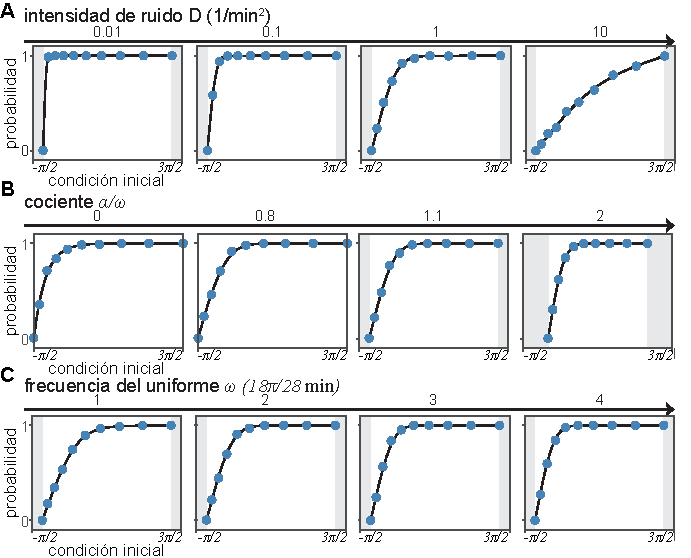
\includegraphics[width=1\columnwidth]{figures/chapter6/C6_eps_plus.pdf} 
    \caption{\textbf{Probabilidad condicional \epsplus(\xx) de llegar a \xxe sin pasar por \xxi en función de la condición inicial \xx.} (A) Probabilidad condicional \epsplus(\xx) en función de su condición inicial \xx para distintos valores de intensidad de ruido, indicados arriba. $\omega = 18\pi/28$, y $\ddelta = 1.1$. (B) Probabilidad condicional \epsplus(\xx) en función de su condición inicial \xx para distintos valores del cociente adimensional \ddelta, indicados arriba. $\omega = 18\pi/28$, y $D = 1$. (C) Probabilidad condicional \epsplus(\xx) en función de su condición inicial \xx para distintos valores de frecuencia del uniforme, indicados arriba. $\ddelta = 1.1$ y $D=1$. (A-C) Los puntos azules indican los resultados de los cálculos numéricos, la línea negra es el resultado de la expresión analítica \ref{C6_eq:mFPT_eps_res}, y los bordes de la región gris indican el punto fijo inestable (izquierda) o estable (derecha) si corresponde. Las simulaciones numéricas fueron $N=500$, con un paso $dt = 10^{-5}$ y una frecuencia de adquisición de $d=1$.}
    \label{C6_fig:mFPT_eps}
\end{figure}



Una vez que encontramos la solución a \ref{C6_eq:mFPT_eps_S4}, estamos en condiciones de comenzar a trabajar con \ref{C6_eq:mFPT_tplus_eq_res} para obtener la expresión analítica del tiempo de primer pasaje condicional medio $\tplus(\xx)$. Como \ref{C6_eq:mFPT_tplus_eq_res} es una ecuación diferencial para la derivada de este producto $ \epstplus(\xx) = \epsplus(\xx) \tplus(\xx) $,  primero obtendremos una expresión para la derivada de este producto, luego integraremos la solución e impondremos las condiciones de contorno \ref{C6_eq:mFPT_tplus_eq_cdc}, para finalmente obtener la expresión analítica de  $\tplus(\xx)$.


Utilizaremos el método de variación constante para dar con una expresión de \Depstplus(\xx). Como primer paso, queremos determinar la solución homogénea $\DepstplusH(\xx)$ de \ref{C6_eq:mFPT_tplus_eq_res}, y
\begin{align}
    0 &= v(\xx) \DepstplusH(\xx)  + D \DDepstplusH(\xx)\\
    \frac{\DDepstplusH(\xx)}{\DepstplusH(\xx)} &= - \frac{v(\xx)}{D}, 
\end{align}
y
\begin{align}
   \DepstplusH(\xx) & = K  e^{- \frac{V(\xx)}{D}},
\end{align}
donde $V(\xx)$ es la primitiva de $v(\xx)$ y $K$ es una constante positiva.
Luego, permitimos $K \rightarrow   K(\xx)$ tal que $\Depstplus(\xx) = K(\xx) e^{- \frac{V(\xx)}{D}}$, y buscamos hallar la solución particular de \ref{C6_eq:mFPT_tplus_eq_res}
\begin{align}
    - \epsplus(\xx) &= v(\xx) \Depstplus(\xx) + D \DDepstplus(\xx)\\
    - \epsplus(\xx) &= v(\xx) K(\xx) e^{- \frac{V(\xx)}{D}}  \nonumber \\
    & + D K'(\xx)e^{- \frac{V(\xx)}{D}} - D K(\xx) \frac{v(\xx)}{D} e^{- \frac{V(\xx)}{D}} \\
    - \epsplus(\xx) &=  D K'(\xx)e^{- \frac{V(\xx)}{D}} .
\end{align}
Entonces
\begin{align}
         K'(\xx) = - \frac{\epsplus(\xx)}{D} e^{ \frac{V(\xx)}{D}} .
\end{align}
Para encontrar $K(\xx)$ tomamos un límite de integración arbitrario $\xx_{0}$
\begin{align}
         K(\xx) - K_0 = \frac{-1}{D} \int_{\xx_0}^\xx d\xx' \epsplus(\xx') e^{ \frac{V(\xx')}{D}},
\end{align}
donde $K_0 = K(\xx_0)$. Con este resultado, 
\begin{align}
    \Depstplus(\xx) = \frac{-e^{- \frac{V(\xx)}{D}}}{D} \int_{\xx_0}^\xx d\xx' \epsplus(\xx') e^{ \frac{V(\xx')}{D}} + K_0 \; e^{- \frac{V(\xx)}{D}} .
\end{align}
Luego, 
\begin{align}
   \epstplus(\xx) = \int_{\xx_1}^{\xx} d\xx'  \frac{- e^{- \frac{V(\xx')}{D}} }{D} \int_{\xx_0}^{\xx'} d \xx'' \epsplus(\xx'') e^{ \frac{V(\xx'')}{D}} + K_0 \int_{\xx_1}^{\xx} d\xx'  e^{- \frac{V(\xx')}{D}}  .
\end{align}


Si elegimos $\xx_1 = \xxi$, la integral $\int_{\xx_1 = \xxi}^{\xx} d\xx'  e^{- \frac{V(\xx')}{D}} = N \epsplus(\xx)$, y además se cumple una de las condiciones de contorno \ref{C6_eq:mFPT_tplus_eq_cdc} donde $\epstplus(\xxi) = 0$. Luego,
\begin{align}
   \epstplus(\xx) = \int_{\xx_1}^{\xx} d\xx'  \frac{- e^{- \frac{V(\xx')}{D}} }{D} \int_{\xx_0}^{\xx'} d \xx'' \epsplus(\xx'') e^{ \frac{V(\xx'')}{D}} + N \epsplus(\xx) K_0 .
\end{align}
Si definimos $I_0(\xx) =  \frac{-1}{D} \int_{\xx_0}^\xx d \xx' \epsplus(\xx') e^{ \frac{V(\xx')}{D}}$, 
\begin{align}
   \epstplus(\xx) &= \int_{\xxi}^{\xx} d\xx'  e^{- \frac{V(\xx')}{D}}  I_0(\xx')+  N \; \epsplus(\xx) \; K_0 .
   \label{C6_eq:mFPT_tplus_R1}
\end{align}
Si aprovechamos que $ e^{- \frac{V(\xx)}{D}} = N \epsplus(\xx)'$, podemos reescribir la expresión \ref{C6_eq:mFPT_tplus_R1} usando partes para descomponer el término de la integral,
\begin{align}
   \epstplus(\xx) &= I_0(\xx') N \epsplus(\xx') \Bigg]_{\xxi}^{\xx} - \int_{\xxi}^{\xx} d\xx' N \epsplus(\xx') \Big(\frac{-1}{D} \epsplus(\xx') e^{ \frac{V(\xx')}{D}} \Big) +  N \epsplus(\xx) K_0 \\
            &= I_0(\xx) N \epsplus(\xx) - I_0(\xxi) N \epsplus(\xxi) + \frac{N}{D} \int_{\xxi}^{\xx} d\xx'  \epsplus^2(\xx') e^{ \frac{V(\xx')}{D}} +  N \epsplus(\xx) K_0 \\
            &= I_0(\xx) N \epsplus(\xx) + \frac{N}{D} \int_{\xxi}^{\xx} d\xx'  \epsplus^2(\xx') e^{ \frac{V(\xx')}{D}} +  N \epsplus(\xx) K_0 ,
\end{align}
donde en la última igualdad usamos $\epsplus(\xxi) = 0$. Finalmente, 
\begin{align}
   \epstplus(\xx) &= \big(I_0(\xx)+K_0\big) N \epsplus(\xx) + \frac{N}{D} \int_{\xxi}^{\xx} d\xx'  \epsplus^2(\xx') e^{ \frac{V(\xx')}{D}}. 
\end{align}
Ahora podemos determinar las constantes $K_0$ y $\theta_0$ con las condiciones de contorno.
\begin{align}
   \epstplus(\xxe) &= \big(I_0(\xxe)+K_0\big) N \epsplus(\xxe) + \frac{N}{D} \int_{\xxi}^{\xxe} d\xx'  \epsplus^2(\xx') e^{ \frac{V(\xx')}{D}} = 0\\
   0&=\big(I_0(\xxe)+K_0\big) + \frac{1}{D} \int_{\xxi}^{\xxe} d\xx'  \epsplus^2(\xx') e^{ \frac{V(\xx')}{D}} \\
   0&=\frac{-1}{D} \int_{\xx_0}^{\xxe} d \xx' \epsplus(\xx') e^{ \frac{V(\xx')}{D}} +K_0 + \frac{1}{D} \int_{\xxi}^{\xxe} d\xx'  \epsplus^2(\xx') e^{ \frac{V(\xx')}{D}} \\
   K_0 &= \frac{1}{D} \Big( \int_{\xx_0}^{\xxe} d \xx' \epsplus(\xx') e^{ \frac{V(\xx')}{D}} - \int_{\xxi}^{\xxe} d\xx'  \epsplus^2(\xx') e^{ \frac{V(\xx')}{D}}\Big)
\end{align}
Si elegimos $\xx_0 = \xxe$,
\begin{align}
   K_0 &= \frac{-1}{D} \int_{\xxi}^{\xxe} d\xx'  \epsplus^2(\xx') e^{ \frac{V(\xx')}{D}}.
\end{align}
Para terminar, ya tenemos nuestro resultado 
\begin{align}
   \epstplus(\xx) &= \frac{-N}{D} \epsplus(\xx) \Big(  \int_{\xx_e}^\xx d \xx' \epsplus(\xx') e^{ \frac{V(\xx')}{D}} +  \int_{\xxi}^{\xxe} d\xx'  \epsplus^2(\xx') e^{ \frac{V(\xx')}{D}} \nonumber \\ & - \frac{1}{\epsplus(\xx)} \int_{\xxi}^{\xx} d\xx'  \epsplus^2(\xx') e^{ \frac{V(\xx')}{D}} \Big)\\
     \epstplus(\xx) &= \frac{N}{D} \epsplus(\xx) \Big(  \int_\xx^{\xx_e} d \xx' \epsplus(\xx') e^{ \frac{V(\xx')}{D}} -  \int_{\xxi}^{\xxe} d\xx'  \epsplus^2(\xx') e^{ \frac{V(\xx')}{D}} \nonumber \\ & + \frac{1}{\epsplus(\xx)} \int_{\xxi}^{\xx} d\xx'  \epsplus^2(\xx') e^{ \frac{V(\xx')}{D}} \Big)
\end{align}
Finalmente, logramos tener la expresión para el tiempo de primer pasaje condicional medio
\begin{align}
     \tplus(\xx)&= \frac{N}{D} \Big(  \int_\xx^{\xx_e} d \xx' \epsplus(\xx') e^{ \frac{V(\xx')}{D}} -  \int_{\xxi}^{\xxe} d\xx'  \epsplus^2(\xx') e^{ \frac{V(\xx')}{D}} + \frac{1}{\epsplus(\xx)} \int_{\xxi}^{\xx} d\xx'  \epsplus^2(\xx') e^{ \frac{V(\xx')}{D}} \Big) \label{C6_eq:mFPT_tplus_res}
\end{align}

Si tomamos el límite del oscilador uniforme \ref{C6_eq:mFPT_uniforme}, el tiempo de primer pasaje condicional medio es 
\begin{align}
     \tplus(\xx)& = \frac{2 \pi \left(e^{\frac{2 \pi \omega}{D}}+1\right) \left(e^{\frac{\omega \xx}{D}}-1\right)-\xx\left(e^{\frac{2 \pi\omega}{D}}-1\right) \left(e^{\frac{\omega \xx}{D}}+1\right)}{\omega \left(e^{\frac{2 \pi \omega}{D}}-1\right) \left(e^{\frac{\omega \xx}{D}}-1\right)},
     \label{C6_eq:mFPT_tplus_res_alpha_cero} 
\end{align}
expresión que coincide con resultados previamente reportados \cite{Redner2001}. De esta expresión, es interesante notar que cuando la intensidad de ruido tiende a cero, \ref{C6_eq:mFPT_tplus_res_alpha_cero} tiende a $\frac{2\pi - \xx}{\omega}$, y cuando la condición inicial es $0$, el tiempo coincide con el período del oscilador uniforme. Luego, el segundo término de \ref{C6_eq:mFPT_tplus_res_alpha_cero} es la corrección correspondiente a empezar en cualquier lugar \xx del círculo. 


Para corroborar \ref{C6_eq:mFPT_tplus_res}, medimos en simulaciones computacionales cuánto tiempo tardaba el sistema cuya dinámica estaba gobernada por la ecuación \ref{C6_eq:adler_white_noise} e inicialmente se encontraba en \xx en llegar a \xxe. Descartamos todas las mediciones realizadas sobre las trayectorias que atravesaban \xxi (ver apéndice \ref{C6_ap:traces}). En la figura \ref{C6_fig:mFPT_tplus} observamos que nuestra expresión coincide con las simulaciones. Observamos, además, que en todos los casos el tiempo de primer pasaje medio condicional decrece conforme aumenta la condición inicial. Además, si la condición inicial tiende a ser el punto fijo inestable, el tiempo es finito y depende de los parámetros del modelo. 


En \ref{C6_fig:mFPT_tplus}A podemos observar que el ruido tiende a disminuir el tiempo de primer pasaje condicional medio. En \ref{C6_fig:mFPT_tplus}B observamos que el cociente adimensional \ddelta tiene el mismo efecto, pues la velocidad que el sistema puede tener en el intervalo $[\xxi,\xxe]$ aumenta con el cociente \ddelta, así como la distancia entre la condición inicial \xx y el punto fijo estable. De manera similar, un aumento de la frecuencia del uniforme conduce a velocidades mayores que el sistema puede tomar en el intervalo $[\xxi,\xxe]$, que termina aplanando la curva del tiempo de primer pasaje medio condicional (figura \ref{C6_fig:mFPT_tplus}C). 


\begin{figure}
    \centering
    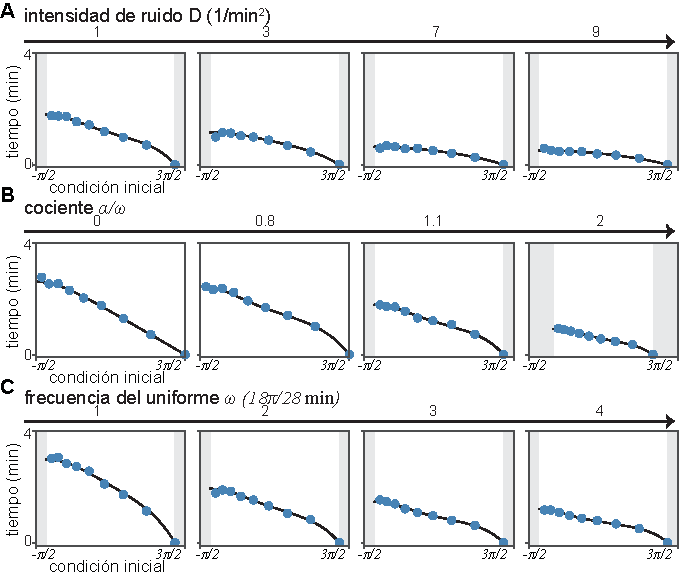
\includegraphics[width=1\columnwidth]{figures/chapter6/C6_t_plus.pdf} 
    \caption{\textbf{Tiempo medio \tplus(\xx) para llegar al punto fijo estable \xxe sin pasar por el punto fijo inestable \xxi en función de la condición inicial \xx.} (A) Tiempo medio \tplus(\xx) en función de su condición inicial \xx para distintos valores de intensidad de ruido. $\omega = 18\pi/28$, y $\ddelta = 1.1$. (B) Tiempo medio \tplus(\xx) en función de su condición inicial \xx para distintos valores del cociente adimensional \ddelta. $\omega = 18\pi/28$, y $D = 1$. (C) Tiempo medio \tplus(\xx) en función de su condición inicial \xx para  distintos valores de frecuencia del uniforme. $\ddelta = 1.1$ y $D=1$. (A-C) Los puntos azules indican los resultados de los cálculos numéricos, la línea negra indica el resultado de la expresión analítica \ref{C6_eq:mFPT_tplus_res}, y los bordes de la región gris indican el punto fijo inestable (izquierda) o estable (derecha) si corresponde. Las simulaciones numéricas fueron $N=500$, con un paso $dt = 10^{-5}$ y una frecuencia de adquisición de $d=1$.}
    \label{C6_fig:mFPT_tplus}
\end{figure}

\subsection{Expresión analítica para la duración de pulsos media}
\sectionmark{Duración de pulsos media}

En la sección anterior observamos que el límite \ref{C6_eq:Txi_def} que define la duración de pulsos media del sistema \ref{C6_eq:adler_white_noise} es finito y depende de los parámetros del modelo. En esta sección queremos obtener una expresión analítica para la duración de pulsos media $T_\xi$, que definimos como el tiempo medio que tarda el sistema en llegar a \xxe, habiendo salido pero nunca vuelto a pasar por \xxi.


Comenzamos por reescribir la ecuación \ref{C6_eq:mFPT_tplus_res} para tener una expresión con límites de integración más sencillos,
\begin{align}
     \tplus(\xx)&= \frac{N}{D} \Big(  \int_\xx^{\xx_e} d \xx' \epsplus(\xx') e^{ \frac{V(\xx')}{D}} -  \int_{\xxi}^{\xxe} d\xx'  \epsplus^2(\xx') e^{ \frac{V(\xx')}{D}} \nonumber \\ & + \frac{1}{\epsplus(\xx)} \int_{\xxi}^{\xx} d\xx'  \epsplus^2(\xx') e^{ \frac{V(\xx')}{D}} \Big) \\
     &= \frac{N}{D} \Big[  \int_\xx^{\xx_e} d \xx' \epsplus(\xx') e^{ \frac{V(\xx')}{D}} \big(1 - \epsplus(\xx') \big)+ \nonumber \\ & \big( \frac{1}{\epsplus(\xx)} -1 \big) \int_{\xxi}^{\xx} d\xx'  \epsplus^2(\xx') e^{ \frac{V(\xx')}{D}} \Big]. \label{C6_eq:Txi_tplus_terminos}
\end{align}

Tenemos una expresión que es la suma de dos integrales. Comenzaremos por trabajar con el primer término 
\begin{align}
     \lim_{\xx \rightarrow   \xxi }&\frac{N}{D}  \int_\xx^{\xxe} d \xx' \epsplus(\xx') e^{ \frac{V(\xx')}{D}} \big(1 - \epsplus(\xx') \big) \\
     &= \frac{N}{D} \int_{\xxi}^{\xxe} d \xx' \epsplus(\xx') e^{ \frac{V(\xx')}{D}} \big(1 - \epsplus(\xx') \big).
     \label{C6_eq:Txi_LI1}
\end{align}


Luego, detengámonos en el segundo término de \ref{C6_eq:Txi_tplus_terminos}. Es fácil ver que la integral de este término tiende a cero cuando $\xx \rightarrow \xxi $, pues el límite de integración superior tiende al límite de integración inferior. Esto mismo ocurre con \epsplus(\xx). Según su expresión analítica \ref{C6_eq:mFPT_eps_res}, $\epsplus(\xx) \rightarrow 0$ cuando $\xx \rightarrow \xxi $. Esta indeterminación hacen que este límite no sea fácil de calcular. Luego, para determinar el límite del segundo término, es necesario salvar la indeterminación 
\begin{align}
      \lim_{\xx \rightarrow   \xxi }& \frac{1}{\epsplus(\xx)}  \int_{\xxi}^{\xx} d\xx'  \epsplus^2(\xx') e^{ \frac{V(\xx')}{D}}.
     \label{C6_eq:Txi_LI2_S1}
\end{align}
A partir de \ref{C6_eq:mFPT_eps_res}, podemos determinar que 
\begin{align}
     \epsplus'(\xx) & = \frac{e^{- \frac{V(\xx)}{D}}}{N},
\end{align}
y en particular 
\begin{align}
     \epsplus'(\xxi) & = \frac{e^{- \frac{V(\xxi)}{D}}}{N} = \frac{e^{- \frac{\omega \xxi - \alpha \cos{(\xxi)}}{D}}}{N} \neq 0.
\end{align}
Luego, como $\epsplus'(\xxi)$ no se anula ni en \xxi ni en su entorno, podemos usar la regla de L'Hospital para salvar la indeterminación \ref{C6_eq:Txi_LI2_S1}
\begin{align}
     & \lim_{\xx \rightarrow   \xxi } \frac{1}{\epsplus(\xx)}  \int_{\xxi}^{\xx} d\xx'  \epsplus^2(\xx') e^{ \frac{V(\xx')}{D}}\\
     & = \lim_{\xx \rightarrow   \xxi } \frac{1}{\frac{e^{- \frac{V(\xx)}{D}}}{N}}  \; \epsplus^2(\xx) e^{ \frac{V(\xx)}{D}} \\
     & = \frac{1}{\frac{e^{- \frac{V(\xxi)}{D}}}{N}}  \; \epsplus^2(\xxi) e^{ \frac{V(\xxi)}{D}} \\
     & = \frac{1}{\frac{e^{- \frac{V(\xxi)}{D}}}{N}}  \times 0. 
     \label{C6_eq:Txi_LI2_S2}
\end{align}
Mientras que el primer término de \ref{C6_eq:Txi_LI2_S2} es distinto de cero, su segundo término tiende a cero. Para corroborar este límite, estudiamos el comportamiento de \ref{C6_eq:Txi_LI2_S1} en un entorno de \xxi (figura \ref{C6_fig:Txi_LI2_S2}).

\begin{figure}
    \centering
    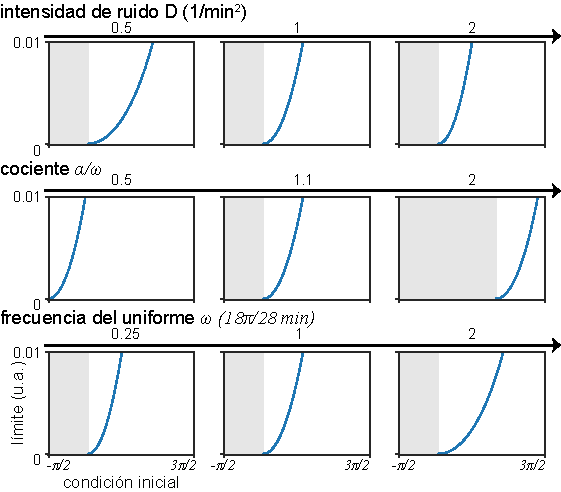
\includegraphics[width=1\columnwidth]{figures/chapter6/C6_limite_int_2.pdf} 
    \caption{\textbf{Comportamiento de \ref{C6_eq:Txi_LI1} cerca del punto fijo inestable \xxi}. Comportamiento de \ref{C6_eq:Txi_LI1} cerca del punto fijo inestable \xxi para distintos valores de la intensidad del ruido $D$, cociente adimensional $\alpha/\omega$ y frecuencia del homogéneo $\omega$ indicados. $\omega = \frac{2\pi}{7 \text{min}}$, $\ddelta = 1.1$ , y $\D = 1 \frac{1}{\text{min}^2}$, a excepción de que se especifique otro valor. Los bordes de la región gris indican el punto fijo inestable si corresponde}
    \label{C6_fig:Txi_LI2_S2}
\end{figure}

Con estos resultados, obtuvimos una expresión analítica para la duración de pulsos
\begin{align}
     T_\xi = \frac{\int_{\xxi}^{\xxe} d \xx' \epsplus(\xx') e^{ \frac{V(\xx')}{D}} \big(1 - \epsplus(\xx') \big)}{D\; \int_{\xxi}^{\xxe} e^{- \frac{V(\xx)}{D}}},
     \label{C6_eq:Txi}
\end{align}
en donde la principal contribución se corresponde al limite \ref{C6_eq:Txi_LI1}.

Para verificar la expresión \ref{C6_eq:Txi}, medimos en simulaciones computacionales cuánto tiempo tardaba el sistema cuya dinámica estaba gobernada por la ecuación \ref{C6_eq:adler_white_noise} e inicialmente se encontraba en \xxi en llegar a \xxe. Descartamos todas las mediciones realizadas sobre las trayectorias que atravesaban \xxi luego del instante inicial (ver apéndice \ref{C6_ap:traces}). En la figura \ref{C6_fig:duration} observamos que nuestra expresión coincide con las simulaciones. 


\begin{figure}
    \centering
    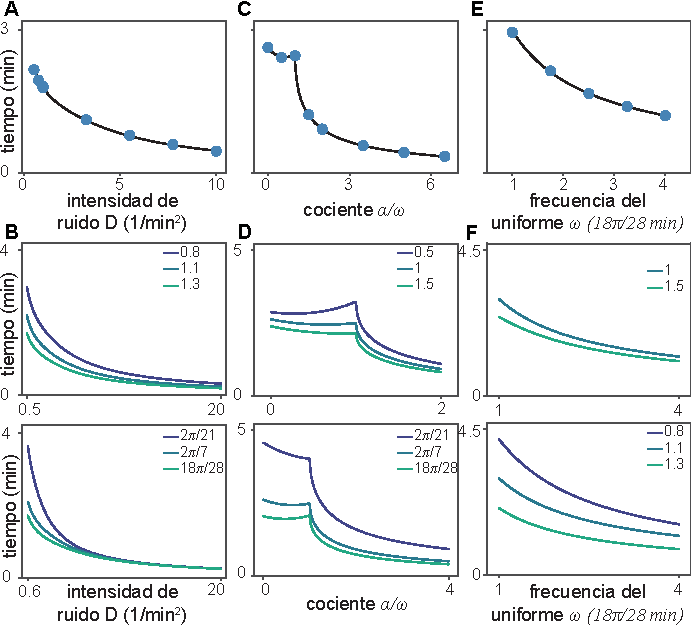
\includegraphics[width=1\columnwidth]{figures/chapter6/C6_duration.pdf} 
    \caption{\textbf{Duración de pulsos $T_\xi$ del modelo de fase con bifurcación de ciclo infinito y ruido blanco gaussiano aditivo.} (A,B) Duración de pulsos $T_\xi$ en función de la intensidad de ruido $D$. En B el cociente adimensional \ddelta (arriba) y la frecuencia del uniforme (abajo, en $1/\text{min}$) se encuentran codificados en escala de colores. (C,D) Duración de pulsos $T_\xi$ en función de el cociente adimensional \ddelta. En D la intensidad de ruido (arriba, en $1/\text{min}^2$) y la frecuencia del uniforme (abajo, en $1/\text{min}$) se encuentran codificados en escala de colores. (E,F) Duración de pulsos $T_\xi$ en función de la frecuencia del uniforme $\omega$. En F la intensidad de ruido (arriba, en $1/\text{min}^2$) y la frecuencia del uniforme (abajo, en $1/\text{min}$) se encuentran codificados en escala de colores (A-F). $\omega = \frac{18\pi}{28 \text{min}}$, $\ddelta = 1.1$ , y $D = 1 \frac{1}{\text{min}^2}$, a excepción de que se especifique otro valor. (A,C,E)  Los puntos azules indican los resultados de los cálculos numéricos, y la línea negra indica el resultado de la expresión analítica \ref{C6_eq:Txi}. Las simulaciones numéricas fueron $N=10^6$, con un paso $dt = 10^{-5}$ y una frecuencia de adquisición de $d=1$.}
    \label{C6_fig:duration}
\end{figure}


En el panel A de la figura \ref{C6_fig:duration} observamos que la duración de pulsos disminuye conforme aumenta el ruido. Además, la escala temporal del comportamiento disminuye conforme aumenta el cociente \ddelta, y la frecuencia del uniforme $\omega$ (figura \ref{C6_fig:duration}B). Es también interesante que para valores altos de intensidad de ruido, las curvas convergen a una duración límite finita. 

En el panel C de la figura \ref{C6_fig:duration} observamos la duración de pulsos en función de \ddelta. Podemos observar una discontinuidad en el comportamiento en $\ddelta = 1$, donde ocurre la bifuración de \textit{saddle node} de ciclo infinito en el modelo determinista del capítulo \ref{ch5}. Para el caso oscilatorio donde $\ddelta < 1$, si la duración de pulsos es creciente o decreciente con \ddelta depende de los parámetros $D$ y $\omega$ (figura \ref{C6_fig:duration}D). En particular, la duración de pulsos en la bifurcación aumenta con el ruido. Es razonable hipotetizar que para valores muy pequeños de ruido la duración de pulsos en el régimen oscilatorio tienda a comportarse según \ref{C5_eq:T_osc}, y en el excitable según \ref{C5_eq:T_exc}. En particular, podemos pensar que con elecciones correctas de $\omega$ y $D$, podemos conseguir duraciones de pulsos similares si variamos $\alpha$ cerca de la bifurcación. En el régimen excitable donde $\ddelta > 1$, la duración de pulsos siempre decrece conforme aumenta \ddelta. 

Observamos que para frecuencias del uniforme cada vez más altas, la duración de pulsos disminuye (figuras \ref{C6_fig:duration} E,F).  


En resumen, observamos que la duración de pulsos del modelo estocástico depende de los parámetros del modelo de una manera no trivial. Observamos analíticamente y con simulaciones computacionales que la duración de pulsos depende del ruido tanto en el caso excitable como en el oscilatorio. Esta dependencia es uniforme, y menores duraciones se consiguen con mayores valores de intensidad de ruido. También hayamos que para valores de ruido y frecuencia del uniforme fijos, variar $\alpha$ en un entorno del valor de bifurcación puede eventualmente conducir a oscilaciones en el régimen oscilatorio, y actividad pulsátil en el régimen excitable, con duraciones de pulso similares cerca de la bifurcación. En principio, esta caracterización es compatible con que haya un conjunto de parámetros que den origen a una duración de pulsos como en la que observamos en los experimentos. En lo próximo, evaluamos concretamente la posibilidad de que el modelo teórico propuesto pueda reproducir la estadística de nuestras mediciones experimentales, para luego calibrarlo y entender qué características de las oscilaciones intermitentes de actividad de ERK es capaz de reproducir. 


\end{document}

